% !TEX root = _yoko.tex
\def\sectionmargin{\vspace{12pt}}
% ==========================================
% プロジェクト予稿（1P）の本文
% ==========================================

\section{はじめに}
近年，音楽や映画といった時系列メディアを対象とした多様な作品分析手法が提案されている.これ
らの分析において，対象作品の視聴や分析方法の検討など，さまざまな要素が含まれるが，場面分けは
多くの分析手法に共通する基盤的な作業である.分析者は場面分けを直感的に行う場合が多く，その基
準は明確化されていないことが多い.

特に映像作品においては，鑑賞者や分析者それぞれが異なる視点を持つため，設定される場面が大き
く異なることが指摘される.このような状況を踏ま
え，本研究では映像作品の場面分けに着目し，場面
を細分化する際に考慮される要素を分析・考察して
いく.
\sectionmargin
\section{研究背景}
時系列メディアを扱った分析はさまざまな手法で
行われている.分析をする上で様々な作業があるが，対象作品の場面分けは多くの分析手法に共通するものである.場面分けの手法として，自動で分割する方法やシステム分割する方法や手動で分割する方法が存在する.

本研究では，手動で分析する際，どのような基準をもって場面分けを行っているか調査を行う.調査方法として，国内の日本語論文に対し，分析者が手動によるメディア分析を対象とした論文を抽出した.分析対象は以下の8つのカテゴリに絞った:演劇，小説，プレゼンテーション，映画，将棋，映像，作品分析，感情分析.これらの論文から，さらに「分析」と「場面分け」に関する記載があるものを抽出し，対象を絞り込んだ.次に，抽出された論文に記載された場面分けに着目し，各分析者がどのような観点や理論に基づいて作品の場面分けを行っているのかを調査を行った.その結果，該当する論文は合計84件が抽出された.そのうち，「分析」と「場面分け」に関する記載が明確に認められる論文は12件に絞られた.
\sectionmargin
\subsection{考察}
論文調査を通じて，分析対象となる作品全体を明
確な理由をもって場面分けしている分析事例は確認
されなかった.この結果から，分析者は場面分けそ
のものを必ずしも重要視しているわけではない可能
性が示唆される.

場面分けは，あくまで分析対象作品のどの部分を指しているかを可視化するための手段として機能しているに過ぎず，その行為自体に特別な意味を持たせる必要性を感じていないと考えられる.そのため，場面分けのプロセスは多くの場合において直感的に行われているのではないかと推察される.
\sectionmargin
\section{同一作品の解釈}
これまでで，さまざまな作品を対象とした分析を
調査したが，同一作品を複数の視点で分析するもの
は存在しなかった.そこで同一作品を複数の視点で
場面分けした場合どのような解釈になるのか疑問に
思った.

そこで同一作品を複数人が場面分けすることで，複数の視点で解釈する方法が可能となるのではないかと考えた.本研究では，場面分けの比較実験を行い分析することで，場面分けをする際どのような要素があるのか考察していく.

\sectionmargin
\subsection{比較分析}
分析方法として，被験者を用意してそれぞれ同じ映像作品を複数話鑑賞してもらい場面分けを行っていく.同一話数の場面分けを比較し，場面分けが同じになる場所や異なる場所を抽出し，なぜそのようなことが起こるのか考察していく（図\ref{fig:hikaku}）．

\begin{figure}[tb]
\centering
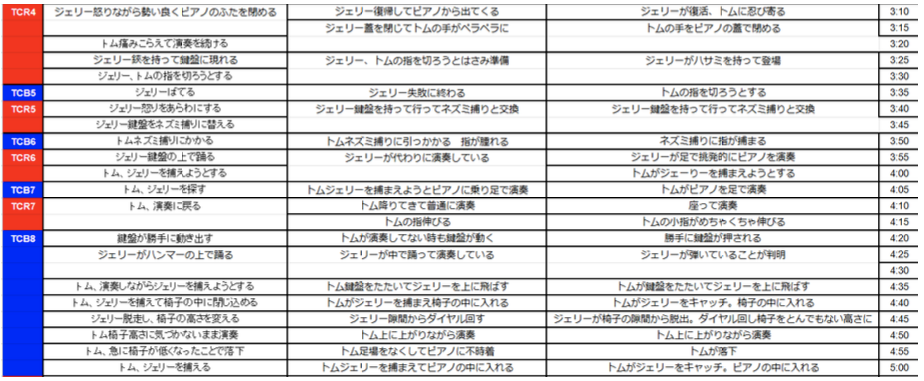
\includegraphics[width=\hsize]{fig/fig.png}
\caption{比較分析例}
\label{fig:hikaku}
\end{figure}

\subsection{対象作品}
1940年から1958年までに公開された短編アニメーションシリーズのトムとジェリー\cite{tom}から4作品を対象とする．トムとジェリーを対象とした理由としては，登場人物が少なく，一話完結で，短編かつ話が数多く存在したためである．対象とする話としては，The Two Mouseketeers・The Cat Concerto・The Missing Mouse・Mouse Troubleの4作品である．


\subsection{場面分けに必要な要素}
調査と分析によって得られた場面分けに必要な要素として物語内の場面の転換，鑑賞者の物語内における視点，行動の細分化，登場人物の感情や行動や関係性，鑑賞者の感情なのではないかと考えた．

\sectionmargin
\section{まとめ}
本研究では，場面分けにたいして調査，比較分
析，考察，提案を行ってきた.調査として作品分析を行っている論文を収集し，
場面分けの現状を調べた.

 そのことを踏まえて短編アニメーション作品のト
ムとジェリーを対象として被験者に場面分けを行っ
てもらい比較，考察を行った.その考察を踏まえて
場面分けに最低限必要な要素として場面転換，鑑賞
者の物型に対する視点，行動の細分化，登場人物の
感情や行動や関係性，鑑賞者の感情ではないかと提
案する.